\documentclass[11pt]{ctexart}
\usepackage{a4}
\usepackage{graphicx}
\usepackage{geometry}
\geometry{a4paper,left=2cm,right=2cm,top=2.5cm,bottom=2.5cm}

\title{几何基础作业3}
\author{无名}
\date{\today}

\begin{document}
\maketitle
\section{做底角为$72^\circ $等腰三角形}
\begin{figure}[htb]\label{f1}
    \begin{center}
        
\includegraphics[width=0.4\linewidth]{01.png}
        \caption{}
    \end{center}
\end{figure}

首先，如图1我们有线段$AB$

\begin{figure}[htb]\label{f2}
    \begin{center}
        
\includegraphics[width=0.6\linewidth]{02.png}
        \caption{}
    \end{center}
\end{figure}

如图2做线段$AB$的中位线，记交$AB$于$O$点。再做线段$OB$的中位线，记交$AB$于$M$点。以O为圆心，$OA$为半径做圆O。
\newpage
\begin{figure}[htb]\label{f3}
    \begin{center}
        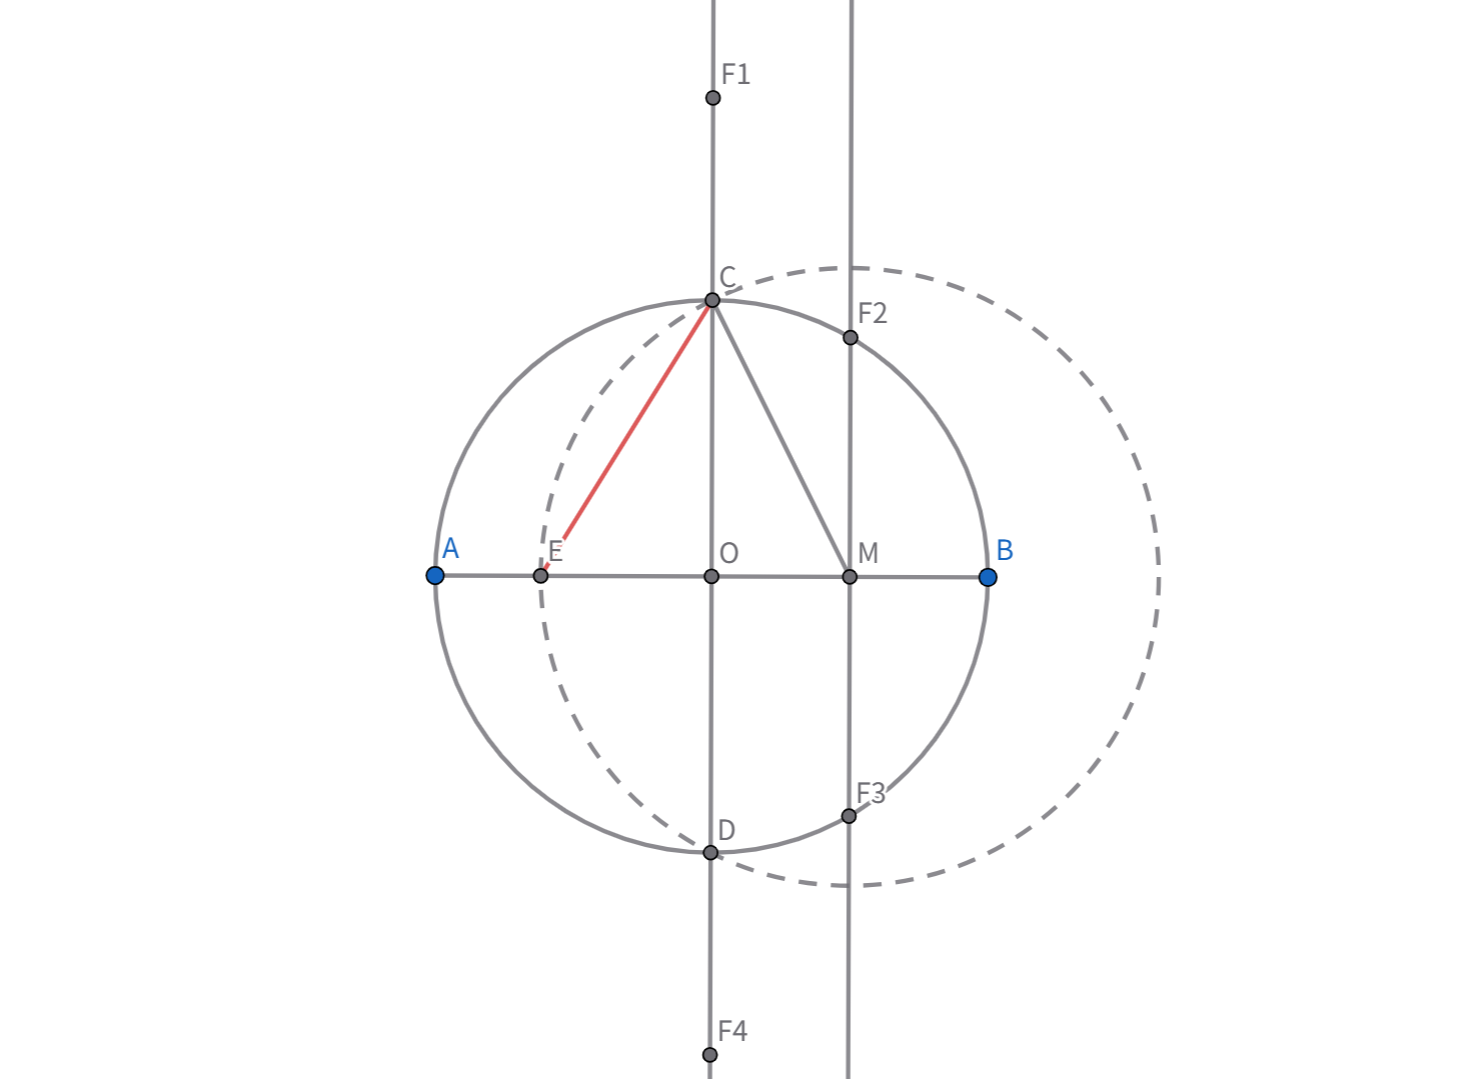
\includegraphics[width=0.6\linewidth]{03.png}
        \caption{}
    \end{center}
\end{figure}

如图3，以M为圆心，$MC$为半径，在$AB$上划弧，交$AB$于E。然后连接$CE$。

\begin{figure}[htb]\label{f4}
    \begin{center}
        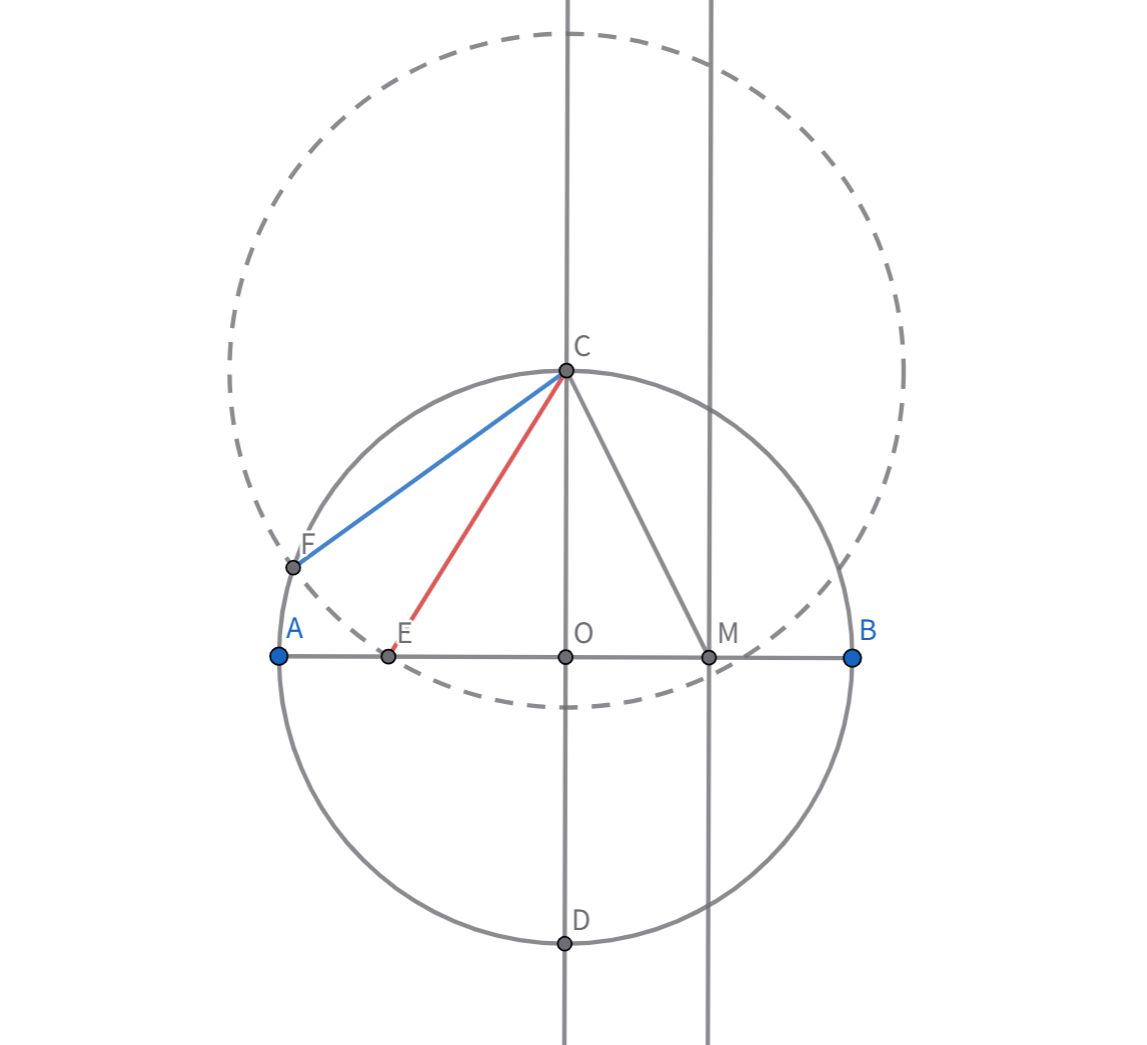
\includegraphics[width=0.5\linewidth]{04.png}
        \caption{}
    \end{center}
\end{figure}

如图4，以C为圆心，$CE$为半径做圆，交$\odot O$于点F
\newpage
\begin{figure}[htb]\label{f5}
    \begin{center}
        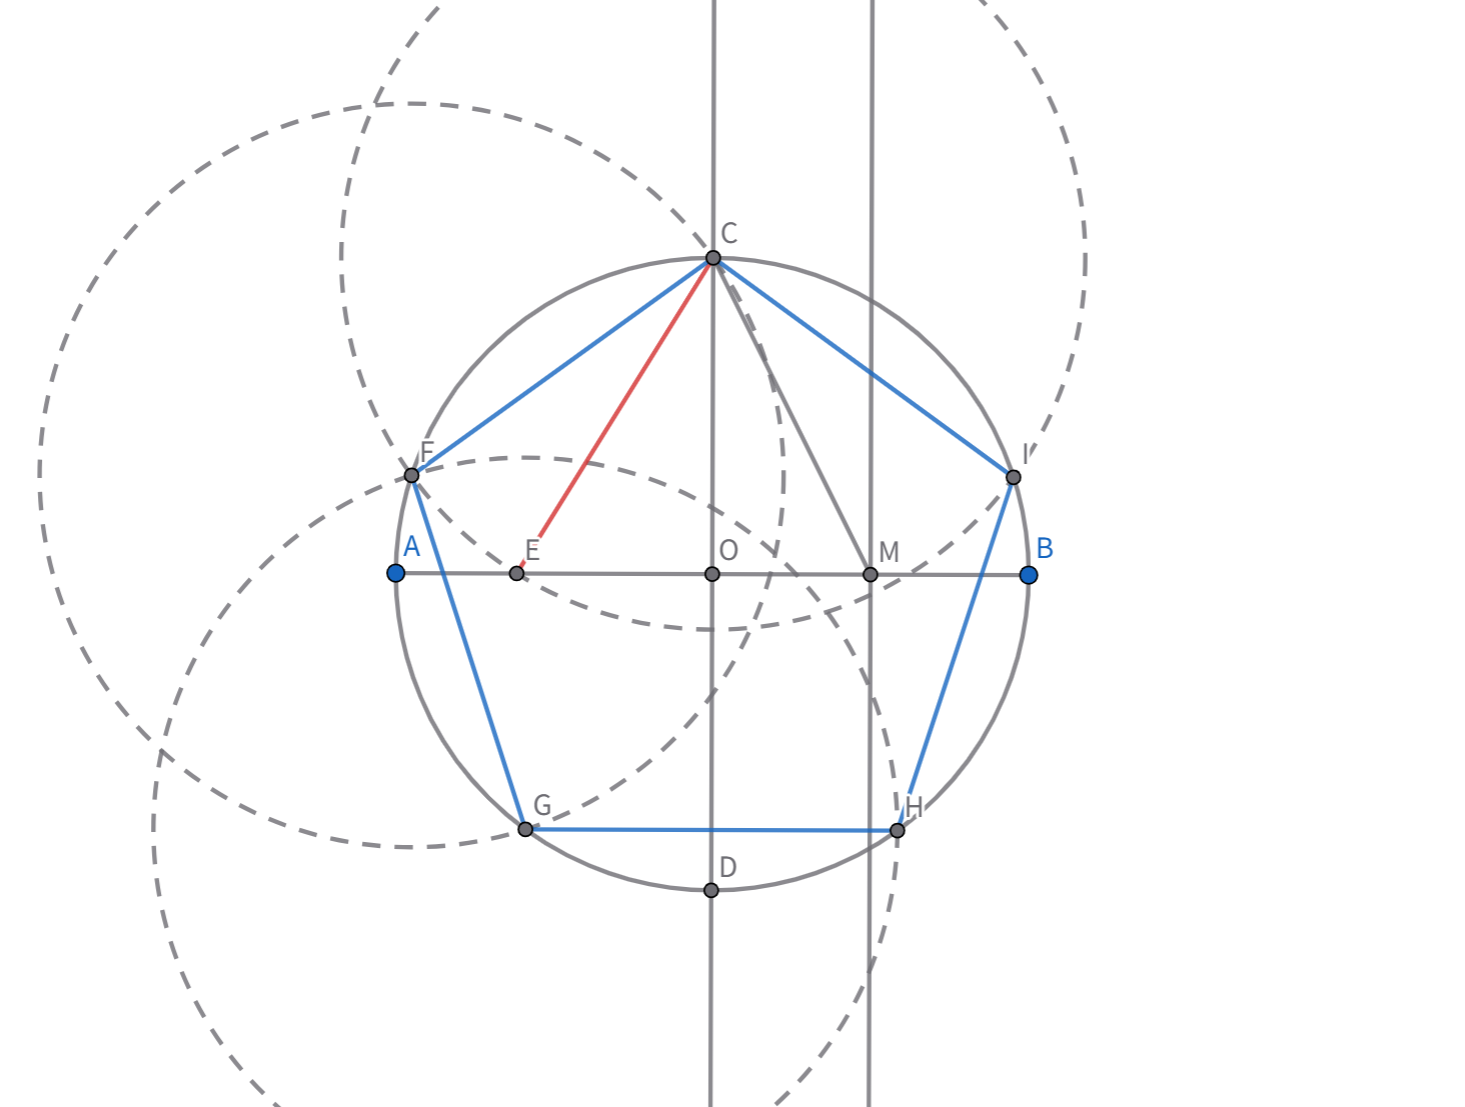
\includegraphics[width=0.6\linewidth]{05.png}
        \caption{}
    \end{center}
\end{figure}

如图5，取$CF$长度重复过程，做出正五边形CFGHI

\begin{figure}[htb]\label{f6}
    \begin{center}
        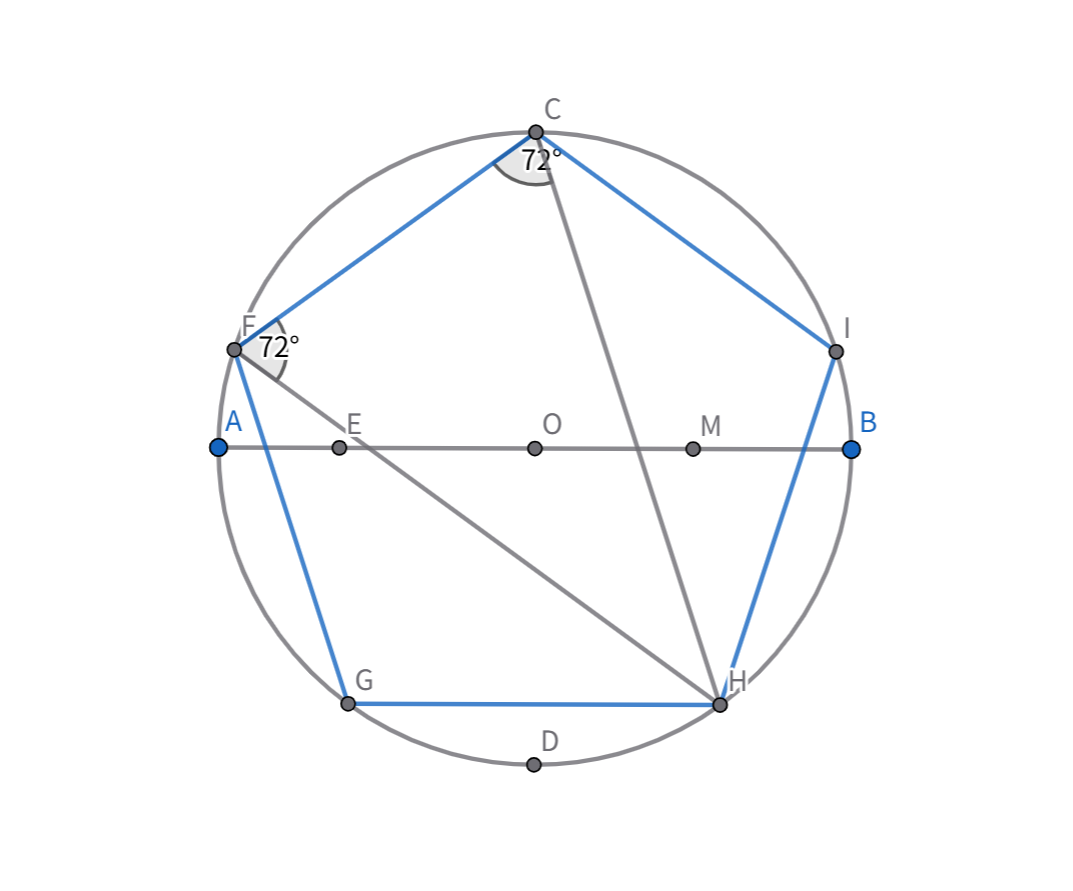
\includegraphics[width=0.5\linewidth]{06.png}
        \caption{}
    \end{center}
\end{figure}

如图6，连接$CH$，$FH$，即得到所作三角形$\bigtriangleup CFH$
\newpage
\section{叙述证明托勒密定理}
\begin{figure}[htb]\label{f7}
    \begin{center}
        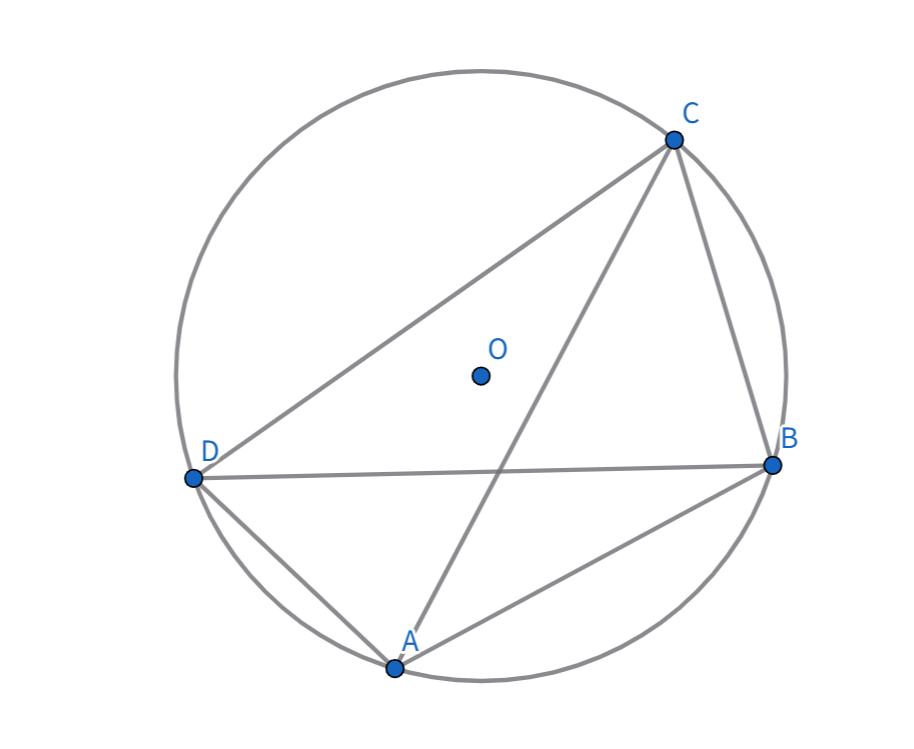
\includegraphics[width=0.5\linewidth]{07.png}
        \caption{}
    \end{center}
\end{figure}
托勒密定理:对于一个内接圆的四边形，四边形的对角线乘积等于两组对边乘积之和

如图7，即为证明:
\[ AC\times BD=AB\times CD + AD\times BC\]

证明：\\
在圆O内，显然$\angle ABC=\angle ADC=\theta $\\
由余弦定理:在$\bigtriangleup ABC$中
\[AC^2=AB^2+BC^2-2AB\cdot BC \cdot \cos \theta \]
在$\bigtriangleup ADC$中
\[AC^2=AD^2+CD^2-2AD\cdot DC \cdot \cos \theta\]
从而
\[\frac{AB^2+BC^2-AC^2}{AB\cdot BC}=\frac{AD^2+CD^2-AC^2}{AD\cdot DC}
\]
\[(AB^2+BC^2)\times AD\cdot DC+(AD^2+CD^2)\times AB\cdot BC=AC^2(AB\cdot BC+AD\cdot DC)
\]
从而
\[AC=\sqrt{\frac{(AB\cdot CD+BC\cdot AD)(AB\cdot AD+BC\cdot CD)}{AB\cdot BC+AD\cdot DC}} \]
同理
\[BD=\sqrt{\frac{(AB\cdot CD+BC\cdot AD)(AB\cdot BC+AD\cdot DC)}{AB\cdot AD+BC\cdot CD}}\]
相乘即有
\[ AC\times BD=AB\times CD + AD\times BC\]
证毕
\end{document}